\section{实验一：资产探查与端口扫描}

\subsection{实验环境与网络拓扑}

本实验在 VirtualBox 中使用 OpenWRT 路由器搭建隔离的资产探测网络。Attacker 位于攻击者网段 \texttt{192.168.2.0/24}，待探测资产位于 \texttt{192.168.4.0/24}，两个网段由 OpenWRT 转发。按照实验指导，在 \texttt{192.168.4.60--192.168.4.70} 的地址范围内布置三台隐藏主机，并保留 \texttt{192.168.4.105} 作为后续全端口扫描的服务器。
各虚拟机在本实验中的地址及角色见表~\ref{tab:task1-network}。

\begin{table}[H]
    \centering
    \caption{资产探查与端口扫描实验的实际网络配置}
    \label{tab:task1-network}
    \renewcommand{\arraystretch}{1.2}
    \begin{tabularx}{\linewidth}{l l X}
        \toprule
        虚拟机 & 实验使用的 IPv4 地址 & 实验角色 \\
        \midrule
        OpenWRT & \texttt{192.168.2.1}、\texttt{192.168.4.1} & 攻击者网段与资产区之间的路由器 \\
        Attacker & \texttt{192.168.2.100} & 资产探测与端口扫描主机 \\
        Victim & \texttt{192.168.4.61} & 隐藏资产 A \\
        User & \texttt{192.168.4.65} & 隐藏资产 B \\
        HostC & \texttt{192.168.4.69} & 隐藏资产 C \\
        Server & \texttt{192.168.4.105} & 待扫描的 Web 服务器 \\
        \bottomrule
    \end{tabularx}
\end{table}

其中，OpenWRT 的 \texttt{eth3} 和 \texttt{eth1} 分别连接攻击者所在的 \texttt{IntNet2} 与资产区所在的 \texttt{IntNet1}。为复用此前的虚拟机环境，Victim、User 通过新增网卡接入资产区，HostC 则直接连接 \texttt{IntNet1}。Attacker 使用 \texttt{enp0s3} 发起探测，经 OpenWRT 到达资产区，因此扫描主机与目标主机不需要处于同一个二层网络。

在 Attacker 上安装实验所需的 \texttt{hping3} 和 \texttt{Nmap}：

\begin{lstlisting}[language=bash,caption={安装资产探测与端口扫描工具}]
sudo apt install -y hping3 nmap
\end{lstlisting}

实际安装结果如图~\ref{fig:task1-install} 所示。

\begin{figure}[H]
    \centering
    
\includegraphics[width=0.90\linewidth]{figures/task12/安装相关工具.png}
    \caption{Attacker 安装 \texttt{hping3} 和 \texttt{Nmap} 工具}
    \label{fig:task1-install}
\end{figure}

\subsection{使用 \texttt{hping3} 进行 ICMP 主机探测}

首先使用 \texttt{hping3} 的 \texttt{-1} 参数发送 ICMP Echo Request，遍历实验指导指定的 \texttt{192.168.4.60--192.168.4.70} 地址范围。若目标主机正常回复 Echo Reply，即可判断其能够响应此次 ICMP 探测。实际操作命令如下：

\begin{lstlisting}[language=bash,caption={使用 ICMP Echo 批量探测隐藏资产}]
for i in {60..70}; do
    echo "========== 192.168.4.$i =========="
    sudo hping3 -1 -I enp0s3 -c 2 192.168.4.$i
done
\end{lstlisting}

这里使用 \texttt{-I enp0s3} 显式指定 Attacker 的网络接口，是因为此前未指定接口时，\texttt{hping3} 曾错误选择回环接口 \texttt{lo}，导致所有目标均无响应。\texttt{-c 2} 表示每个地址只发送两个测试报文，便于观察和比较。

实际扫描只有 \texttt{192.168.4.61}、\texttt{192.168.4.65} 和 \texttt{192.168.4.69} 收到了 ICMP 回复，三台主机均为 2 发 2 收、丢包率为 0\%，对应终端截图分别见图~\ref{fig:task1-icmp-61}、图~\ref{fig:task1-icmp-65}、图~\ref{fig:task1-icmp-69}。

\begin{figure}[H]
    \centering
    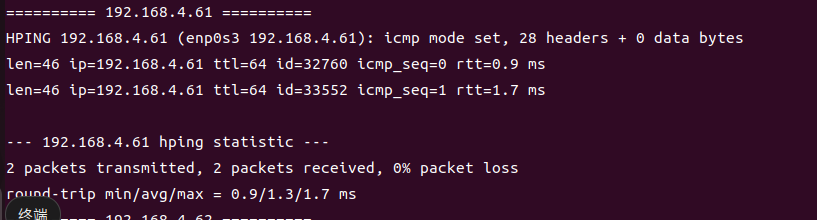
\includegraphics[width=0.86\linewidth]{figures/task12/第一台资产.png}
    \caption{ICMP 探测发现隐藏资产 \texttt{192.168.4.61}}
    \label{fig:task1-icmp-61}
\end{figure}

\begin{figure}[H]
    \centering
    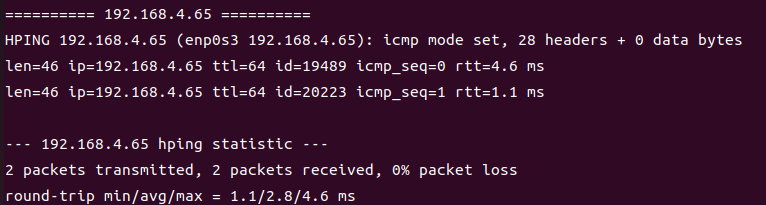
\includegraphics[width=0.86\linewidth]{figures/task12/第二台资产.png}
    \caption{ICMP 探测发现隐藏资产 \texttt{192.168.4.65}}
    \label{fig:task1-icmp-65}
\end{figure}

\begin{figure}[H]
    \centering
    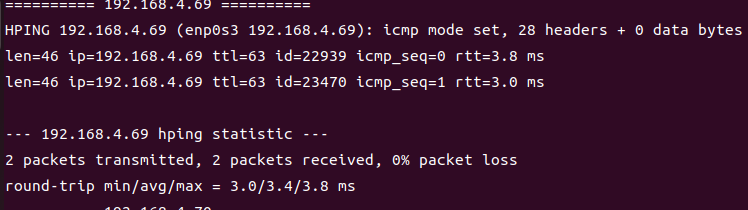
\includegraphics[width=0.86\linewidth]{figures/task12/第三台资产.png}
    \caption{ICMP 探测发现隐藏资产 \texttt{192.168.4.69}}
    \label{fig:task1-icmp-69}
\end{figure}

其余地址在本轮测试中均未收到回复。由此可以确定三台已响应的存活资产，但未收到 ICMP 回复并不必然意味着目标离线，也可能是探测报文被过滤。

\subsection{使用 \texttt{hping3} 进行 TCP 标志位探测}

按照实验指导，先针对 \texttt{192.168.4.61} 的 TCP 80 端口分别发送携带 SYN、ACK、PUSH、FIN、RST 标志位的报文，检查目标的 TCP 响应：

\begin{lstlisting}[language=bash,caption={对单个目标进行五种 TCP 标志位探测}]
sudo hping3 -S -I enp0s3 -p 80 -c 2 192.168.4.61
sudo hping3 -A -I enp0s3 -p 80 -c 2 192.168.4.61
sudo hping3 -P -I enp0s3 -p 80 -c 2 192.168.4.61
sudo hping3 -F -I enp0s3 -p 80 -c 2 192.168.4.61
sudo hping3 -R -I enp0s3 -p 80 -c 2 192.168.4.61
\end{lstlisting}

根据实际终端输出，各类型报文的响应如表~\ref{tab:task1-tcp-flags} 所示。

\begin{table}[H]
    \centering
    \caption{\texttt{192.168.4.61:80} 的 TCP 标志位探测结果}
    \label{tab:task1-tcp-flags}
    \renewcommand{\arraystretch}{1.2}
    \begin{tabularx}{\linewidth}{l c c X}
        \toprule
        发送标志位 & 返回标志位 & 收发结果 & 结果分析 \\
        \midrule
        SYN & RA & 2/2 & 收到 RST+ACK，表明主机有响应，80 端口关闭 \\
        ACK & R & 2/2 & 收到 RST，可说明有 TCP 响应，但无法单独判断端口开闭 \\
        PUSH & RA & 2/2 & 收到 RST+ACK，目标拒绝该报文 \\
        FIN & RA & 2/2 & 收到 RST+ACK，目标拒绝该报文 \\
        RST & 无 & 0/2 & 未收到应答；RST 报文通常不会再触发 TCP 回复 \\
        \bottomrule
    \end{tabularx}
\end{table}

其中，\texttt{flags=RA} 表示响应同时携带 RST 和 ACK 标志，说明目标的 TCP 协议栈确实收到了探测报文，但目标 TCP 80 端口没有建立相应连接。因此，端口关闭和主机离线是不同的概念，不能仅凭 80 端口未开放就认为主机不存在。

随后按照实验要求，对 \texttt{192.168.4.60--192.168.4.70} 整个区间发送 SYN 报文：

\begin{lstlisting}[language=bash,caption={使用 TCP SYN 批量探测资产区}]
for i in {60..70}; do
    echo "========== 192.168.4.$i =========="
    sudo hping3 -S -I enp0s3 -p 80 -c 2 192.168.4.$i
done
\end{lstlisting}

结果显示，\texttt{192.168.4.61}、\texttt{192.168.4.65} 和 \texttt{192.168.4.69} 均返回 \texttt{flags=RA}，每个目标均收到两次响应；区间内其余地址未收到回复。TCP SYN 探测与之前的 ICMP 发现结果一致，确认了三台隐藏主机。

\subsection{使用 \texttt{hping3} 进行 UDP 主机探测}

实验指导还要求通过 UDP 报文进行探测。UDP 是无连接协议，不存在 TCP 的 SYN/SYN-ACK 握手；若目标 UDP 端口没有服务监听，目标主机可能返回 ICMP Port Unreachable 差错报文，因此该响应也可以用来识别存活主机。

指导给出的 UDP 端口号为 \texttt{123456}，但源端口和目的端口字段均为 16 bit，合法端口号范围为 0 至 65535。因此本实验将目的端口改为 \texttt{12345}，实验指导中原参数的截图如图~\ref{fig:task1-udp-correction} 所示。

\begin{figure}[H]
    \centering
    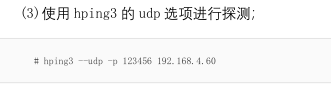
\includegraphics[width=0.73\linewidth]{figures/task12/纠正.png}
    \caption{实验指导中 UDP 目标端口参数的原始写法}
    \label{fig:task1-udp-correction}
\end{figure}

首先探测 \texttt{192.168.4.61}：

\begin{lstlisting}[language=bash,caption={针对单台主机的 UDP 探测}]
sudo hping3 --udp -I enp0s3 -p 12345 -c 2 192.168.4.61
\end{lstlisting}

该主机返回两条 \texttt{ICMP Port Unreachable}，如图~\ref{fig:task1-udp} 所示。该结果表明目标主机可达，但被探测的 UDP 端口未提供可接受该数据报的服务。

\begin{figure}[H]
    \centering
    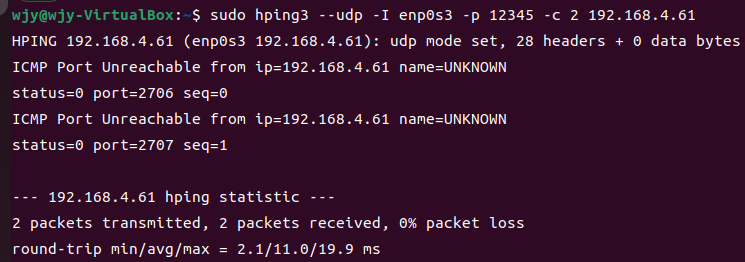
\includegraphics[width=0.84\linewidth]{figures/task12/UDP测试结果.png}
    \caption{对 \texttt{192.168.4.61} 进行 UDP 探测并收到端口不可达响应}
    \label{fig:task1-udp}
\end{figure}

继续遍历完整目标区间：

\begin{lstlisting}[language=bash,caption={UDP 批量主机探测}]
for i in {60..70}; do
    echo "========== 192.168.4.$i =========="
    sudo hping3 --udp -I enp0s3 -p 12345 -c 2 192.168.4.$i
done
\end{lstlisting}

根据实际输出，\texttt{192.168.4.61}、\texttt{192.168.4.65} 和 \texttt{192.168.4.69} 均返回 ICMP Port Unreachable，且各收到两次响应；其他被测地址没有响应。至此，ICMP、TCP SYN 与 UDP 三种方式均探测出相同的三台隐藏主机。需要注意，对于 UDP 探测，无响应同样不能直接等同于主机离线。

\subsection{使用 \texttt{Nmap} 进行主机发现及服务识别}

\subsubsection{资产区主机存活探测}

按照实验指导，使用 \texttt{Nmap} 的 \texttt{-sn} 参数扫描完整资产区 \texttt{192.168.4.0/24}，仅进行主机发现而不执行常规端口扫描：

\begin{lstlisting}[language=bash,caption={Nmap 对整个资产区进行主机发现}]
sudo nmap -sn 192.168.4.0/24
\end{lstlisting}

最终扫描显示共检查 256 个 IP 地址，其中 5 台主机存活，分别为 \texttt{192.168.4.1}、\texttt{192.168.4.61}、\texttt{192.168.4.65}、\texttt{192.168.4.69} 和 \texttt{192.168.4.105}，实际结果如图~\ref{fig:task1-nmap-alive} 所示。

\begin{figure}[H]
    \centering
    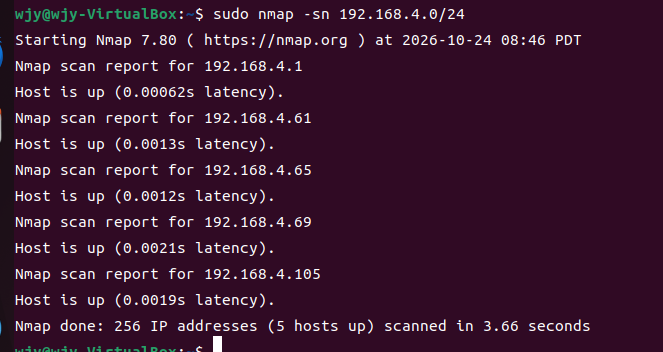
\includegraphics[width=0.84\linewidth]{figures/task12/Nmap结果.png}
    \caption{Nmap 发现资产区中的 5 台存活设备}
    \label{fig:task1-nmap-alive}
\end{figure}

与 \texttt{hping3} 相比，Nmap 一次可以扫描整个网段，并结合多种探测方式判断存活状态。因此，扫描结果不仅包括三台隐藏资产，还包括资产区网关和 Web 服务器。

\subsubsection{操作系统与服务版本识别}

接着按照实验指导使用 TCP SYN 扫描、操作系统识别和服务版本检测：

\begin{lstlisting}[language=bash,caption={Nmap 资产详细信息扫描}]
sudo nmap -sS 192.168.4.0/24 -O -A -sV
\end{lstlisting}

其中，\texttt{-sS} 表示 TCP SYN 扫描，\texttt{-O} 表示操作系统识别，\texttt{-sV} 表示服务版本探测；\texttt{-A} 还会开启版本识别、操作系统检测、默认脚本及路由跟踪等功能。保留这些参数是为了与实验指导中的命令一致。

实际扫描显示：OpenWRT 的 \texttt{22/tcp} 开放 Dropbear SSH 服务，\texttt{53/tcp} 开放 DNS 服务；三台隐藏资产在默认扫描的 1000 个 TCP 端口上均显示为关闭；Web 服务器 \texttt{192.168.4.105} 的 \texttt{80/tcp} 开放 Apache httpd 2.4.52 服务。

需要注意，Nmap 对多个目标报告 \texttt{No exact OS matches} 或 \texttt{Too many fingerprints match this host}，未能精确识别操作系统。因此下文的操作系统名称应结合虚拟机实际部署情况填写，不能将其表述为 Nmap 独立识别的结果。

\subsection{服务器全 TCP 端口扫描}

最后按照实验指导，对目标服务器 \texttt{192.168.4.105} 进行全端口扫描：

\begin{lstlisting}[language=bash,caption={服务器 65535 个 TCP 端口扫描}]
sudo nmap 192.168.4.105 -p- -O -A -sV
\end{lstlisting}

其中 \texttt{-p-} 指定扫描全部 65535 个 TCP 端口，而不是 Nmap 默认选择的常见端口。此次扫描的关键输出如下：

\begin{lstlisting}[caption={服务器全端口扫描的实际关键输出}]
Nmap scan report for 192.168.4.105
Host is up (0.0014s latency).
Not shown: 65534 closed ports
PORT   STATE SERVICE VERSION
80/tcp open  http    Apache httpd 2.4.52
|_http-server-header: Apache/2.4.52 (Ubuntu)
|_http-title: 401 Unauthorized
\end{lstlisting}

由此可知，服务器的 65535 个 TCP 端口中仅 \texttt{80/tcp} 开放，其余 65534 个端口均处于关闭状态。HTTP 检测返回 \texttt{401 Unauthorized}，说明 Apache 服务能够接收并回应请求，但当前访问需要身份认证，并不表示 Web 服务未启动。

\subsection{资产及端口信息统计}

\subsubsection{资产信息统计}

根据主机发现和详细扫描结果，并结合实验环境中实际部署的系统类型，填写实验指导中的资产信息统计表，如表~\ref{tab:task1-assets} 所示。

\begin{table}[H]
    \centering
    \caption{资产信息统计}
    \label{tab:task1-assets}
    \renewcommand{\arraystretch}{1.2}
    \begin{tabularx}{\linewidth}{l l X}
        \toprule
        存活主机 IP & 设备类型 & 操作系统 \\
        \midrule
        \texttt{192.168.4.1} & 路由器 & OpenWRT（Linux） \\
        \texttt{192.168.4.61} & 普通主机（Victim） & Ubuntu Linux \\
        \texttt{192.168.4.65} & 普通主机（User） & Ubuntu Linux \\
        \texttt{192.168.4.69} & 普通主机（HostC） & Ubuntu Linux \\
        \texttt{192.168.4.105} & Web 服务器 & Ubuntu Linux \\
        \bottomrule
    \end{tabularx}
\end{table}

其中操作系统信息来自已知虚拟机部署情况；Nmap 本次只完成了存活主机及部分服务的识别，没有对所有主机给出精确的操作系统指纹结论。

\subsubsection{服务器端口信息统计}

服务器全端口扫描结果对应实验指导中的端口信息统计表，见表~\ref{tab:task1-ports}。

\begin{table}[H]
    \centering
    \caption{服务器 \texttt{192.168.4.105} 的端口信息统计}
    \label{tab:task1-ports}
    \renewcommand{\arraystretch}{1.2}
    \begin{tabularx}{\linewidth}{l l X}
        \toprule
        统计项目 & \texttt{80/tcp} & 其余 65534 个 TCP 端口 \\
        \midrule
        开放状态 & open（开放） & closed（关闭） \\
        服务及版本 & Apache httpd 2.4.52 & 无开放服务 \\
        \bottomrule
    \end{tabularx}
\end{table}

本实验通过 \texttt{hping3} 的 ICMP、TCP、UDP 三类探测发现了三台隐藏资产，再利用 Nmap 识别资产区的五台存活设备，并确认 Web 服务器只开放 \texttt{80/tcp} 端口。三种协议得到的主机发现结果一致，但依赖的响应机制不同；在分析探测结果时，应将主机存活、端口状态和服务版本分别判断。
